\documentclass[border=3pt]{standalone}
% Preâmbulo compartilhado pelos diagramas TikZ da aula 5 de IHC (Processos de Design)
\usepackage[T1]{fontenc}
\usepackage[utf8]{inputenc}
\usepackage{lmodern}
\usepackage{amsmath}
\usepackage{xcolor}
\usepackage{tikz}
\usetikzlibrary{arrows.meta,angles,quotes,decorations.pathmorphing,calc,
                positioning,shapes.geometric,shapes.misc,backgrounds,fit,
                math}

% Paleta (mesma dos SVGs originais)
% Paleta da disciplina de IHC: acento roxo (#755099), da capa do livro.
% (o nome "dblue" é mantido para não alterar todos os diagramas)
\definecolor{dblue}{HTML}{755099}
\definecolor{dorange}{HTML}{B3541E}
\definecolor{dgreen}{HTML}{4A7C59}
\definecolor{dred}{HTML}{9C4B4B}
\definecolor{dcream}{HTML}{F4F1EA}
\definecolor{dshade}{HTML}{DDD7C9}

% Função gaussiana (não normalizada por padrão de escala visual)
\pgfmathdeclarefunction{gauss}{3}{%
  \pgfmathparse{1/(#3*sqrt(2*pi))*exp(-((#1-#2)^2)/(2*#3^2))}%
}

% Estilos comuns (prefixo d... para não colidir com chaves internas do pgf)
\tikzset{
  >={Stealth[length=2mm]},
  dguide/.style={gray!55, dashed, line width=0.4pt},
  daxis/.style={gray!60, line width=0.7pt, ->},
  dbody/.style={fill=black!3, draw=black!80, line width=1pt},
  dacc/.style={draw=dblue, line width=1pt},
  dlbl/.style={black!55, font=\small},
  dsub/.style={black!45, font=\footnotesize},
  dstate/.style={circle, draw=black!80, fill=dcream, line width=1pt,
                 minimum size=17mm, font=\large, inner sep=1pt},
  dobs/.style={circle, draw=black!80, fill=dshade, line width=1pt,
               minimum size=14mm, font=\large, inner sep=1pt},
  dbox/.style={rounded corners=2pt, draw=black!80, fill=dcream, line width=1pt,
               align=center, inner sep=6pt},
  dop/.style={circle, draw=black!80, fill=white, line width=1pt,
              minimum size=6mm, inner sep=0pt, font=\small},
  dtrans/.style={->, dblue, line width=1pt},
  dmeas/.style={->, dorange, line width=1pt},
  dcurve/.style={line width=1pt, dblue},
  dcurveb/.style={line width=1.4pt, dorange},
}

\begin{document}
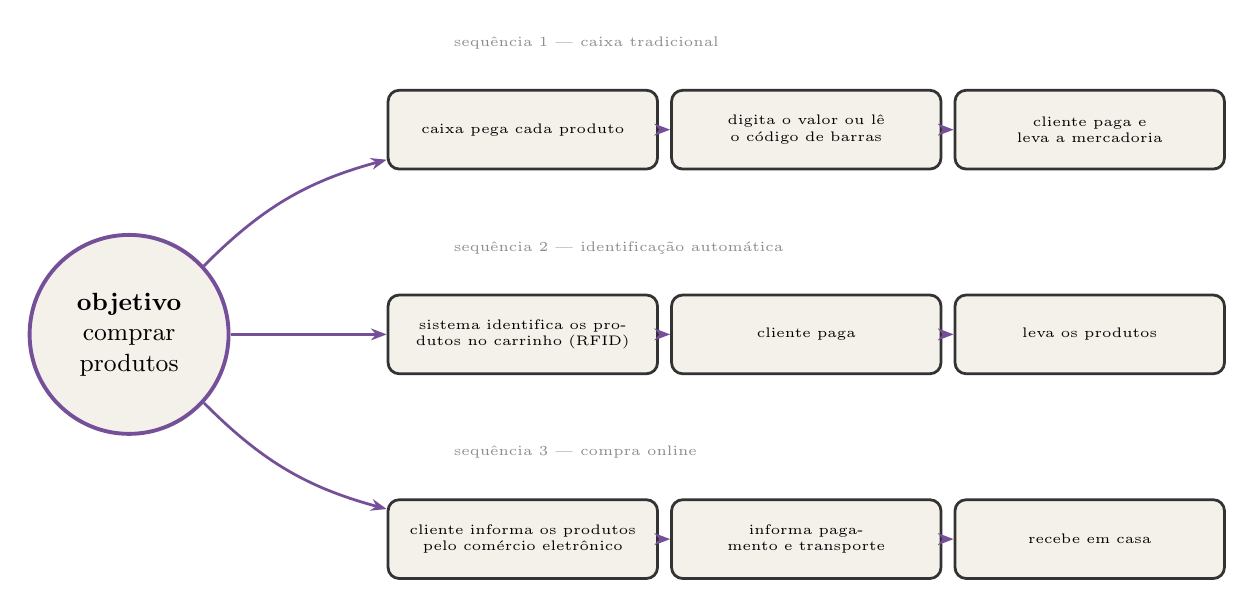
\begin{tikzpicture}[x=1cm,y=1cm,
   t/.style={dbox, rounded corners=4pt, text width=3.0cm, minimum height=1.0cm, font=\tiny}]

  \node[dstate, minimum size=24mm, font=\small, text width=2.2cm, align=center, draw=dblue, line width=1.4pt] (o) at (0,0) {\textbf{objetivo}\\comprar produtos};

  % tarefa 1
  \node[t] (a1) at (5.0,2.6) {caixa pega cada produto};
  \node[t] (a2) at (8.6,2.6) {digita o valor ou lê o código de barras};
  \node[t] (a3) at (12.2,2.6) {cliente paga e leva a mercadoria};
  \draw[dtrans] (o) to[bend left=15] (a1); \draw[dtrans] (a1) -- (a2); \draw[dtrans] (a2) -- (a3);
  \node[dsub, font=\tiny, anchor=west] at (4.0,3.7) {sequência 1 --- caixa tradicional};

  % tarefa 2
  \node[t] (b1) at (5.0,0) {sistema identifica os produtos no carrinho (RFID)};
  \node[t] (b2) at (8.6,0) {cliente paga};
  \node[t] (b3) at (12.2,0) {leva os produtos};
  \draw[dtrans] (o) -- (b1); \draw[dtrans] (b1) -- (b2); \draw[dtrans] (b2) -- (b3);
  \node[dsub, font=\tiny, anchor=west] at (4.0,1.1) {sequência 2 --- identificação automática};

  % tarefa 3
  \node[t] (c1) at (5.0,-2.6) {cliente informa os produtos pelo comércio eletrônico};
  \node[t] (c2) at (8.6,-2.6) {informa pagamento e transporte};
  \node[t] (c3) at (12.2,-2.6) {recebe em casa};
  \draw[dtrans] (o) to[bend right=15] (c1); \draw[dtrans] (c1) -- (c2); \draw[dtrans] (c2) -- (c3);
  \node[dsub, font=\tiny, anchor=west] at (4.0,-1.5) {sequência 3 --- compra online};


\end{tikzpicture}
\end{document}
